\documentclass{article} % For LaTeX2e
\usepackage[final]{../colm2025_conference}

\usepackage{microtype}
\usepackage{hyperref}
\usepackage{url}
\usepackage{amsthm}
\usepackage{amsmath}
\usepackage{amssymb}
\usepackage{pifont}% http://ctan.org/pkg/pifont
\usepackage{booktabs}
\usepackage{soul}
\usepackage{cancel}
\usepackage{algorithm}
\usepackage{algpseudocode}
\usepackage{graphicx}
\usepackage{subfig}
\usepackage{tablefootnote}
\usepackage{multicol}
\theoremstyle{definition}
\newtheorem{theorem}{Theorem}[section]
% \newtheorem{proof}{Proof}[section]

\usepackage{lineno}
\newcommand{\cmark}{\ding{51}}%
\newcommand{\xmark}{\ding{55}}%

\definecolor{darkblue}{rgb}{0, 0, 0.5}
\hypersetup{colorlinks=true, citecolor=darkblue, linkcolor=darkblue, urlcolor=darkblue}


\title{Week 12: Final Summary of RLVR}

\author{\textbf{BEH} Chuen Yang}

\newcommand{\fix}{\marginpar{FIX}}
\newcommand{\new}{\marginpar{NEW}}

\begin{document}

\ifcolmsubmission
\linenumbers
\fi

\maketitle
% - Congrats on finishing the LLM RL training and implementing your own task!
% - In the final two weeks, let’s explore a little bit more on LLM RL and wrap up this project in a report.
% (week 12, you can finish the coding and experiments without writing the report; you can put the results in the final report) 
% Continuing the GSM8k task, let’s consider another reward function. 
% Now we not only want the LLM output formatted and correct answer, we also want the answer to be as short / concise as possible. 
% Design the reward function, run the experiments, and compare with your old runs with analysis.

% - Lastly, write a final report for the WHOLE project. Make it short (<= 5 pages without references). 
% Make it comprehensive (include introduction, method, experiments, and conclusion;
% mirror a research paper that you read.).
%  A tip is that you can copy-paste from your previous report about the RL equations, LLM basics and so on, and summarize them in a concise way.
% Please include the experimental results of week 12 in the report.
% There’s no need to submit at the end of week 12; you can submit the code and final report at the end of week 13.

\begin{abstract}
    This final report summarizes the work done throughout the past weeks on Reinforcement Learning (RL), Large Language Models (LLMs),
    and RL with Verifiable Rewards (RLVR) in LLMs.
    Leaving the intermediate work aside, this report presents most of the key results and findings from all weeks of the project.
    We hope the report serves as a good roadmap for understanding RLVR and how it can be implemented in LLMs.
\end{abstract}

\section{Introduction}
Large Language Models (LLMs) have long been demonstrated capable of performing a staggering variety of tasks
in the Natural Language Processing (NLP) domain, ranging from text generation, 
sentiment analysis, to machine translation, question answering (\cite{Brown-et-al-2020}),
and in recent years, even complex reasoning tasks (\cite{tulu3, grpo, r1}).

% It goes without saying, then, that being able to peer behind the curtain of such a powerful
% and apparently generalized model will be a fascinating endeavor. 
By gaining a deeper
% and more minute 
understanding of how LLMs work, what they are capable of,
and what their limitations are, we will be able to harness their power
in more suitable and effective ways, and even expand the boundaries 
of what is possible with deep learning in general.

% In this brief paper, we present an executive summary of the prerequisite background
% in Reinforcement Learning (RL) and LLMs, highlighting key concepts and findings from our work \footnote{
%     These works will not be cited in-line for brevity,
%     but can be found in the references section at the end of this report.
%     The reader should keep in mind that the previous works serve as the foundation
%     for the current report, and can be referenced for more in-depth treatments
%     of their respective topics.
% },
% and progressively \textit{build up to a high-level overview of RL with Verifiable Rewards (RLVR) in LLMs},
% which is the main focus of this report.
% We supplement our descriptions and theorywork with experimental results
% from past weeks, in order to scaffold a more comprehensive understanding
% of how RL, LLM training, and RLVR work in practice, as well as how and where
% they may fall short.

\section{Background}

The following informally summarize the key concepts necessary to understand
RLVR. More details can be found in the Appendices (where applicable)
as well as in previous weeks' works.

\subsection{LLMs}
As their name partly suggests, LLMs are a class of neural networks 
which attempt to learn the statistical distribution of natural language
(\cite{Zhao-et-al-2023, Karpathy-2025}). Especially in the modern context,
LLMs are \textbf{by and large} \footnote{Exceptions exist and are mentioned in \cite{wk5}. They are omitted here for brevity.} characterized by the following properties (\cite{wk5}):
\begin{itemize}
    \item LLMs model language \textit{causally} (\cite{Jurafsky-2024, Karpathy-2025}).
    \item LLMs adopt \textit{some variant of the Transformer architecture} (\cite{Vaswani-et-al-2017}).
    \item LLMs require a lot of data (often in the tens of terabytes (\cite{Karpathy-2025})) to train.
    \item LLMs typically have \textit{billions or even trillions} of parameters.
    \item Modern LLMs typically have \textit{diverse capabilities}, (\cite{Brown-et-al-2020})
        such as generating coherent text, following instructions, 
        and even engaging in conversations.
\end{itemize}

\subsubsection{How are LLMs trained?}
Per \cite{Karpathy-2025}, LLMs typically undergo multiple stages of training,
developing different capabilities at each stage.

Firstly, during \textit{pre-training}, LLMs are trained on a large corpus of text data
to learn general language patterns and structures by optimizing the objective in Equation \eqref{eq:pretrain-obj}.
This stage is typically \textit{self-supervised} in that the corpus
provides both the conditioning context and the target output, eliding
the need for human-curated labels. See Appendix \ref{sec:cs-nanogpt} and (\cite{wk8})
for an experiment on pre-training a small LLM on the TinyShakespeare corpus (\cite{tinyss, tinyss2}).

Next, some LLMs (\cite{InstructGPT-2022}) undergo \textit{supervised fine-tuning} on more specialized corpora to adapt 
their capabilities to specific tasks or domains (\cite{radford-et-al-2019,Brown-et-al-2020}).
While the objective is identical to Equation \eqref{eq:pretrain-obj} (\cite{wk5}),
the corpus \textit{consists of human-annotated examples} and 
the objective \textit{does not consider the log-likelihoods of the prompt tokens} (
    since strictly speaking, the prompt tokens are not part of the target output
).

Finally, most modern LLMs (\cite{tulu3, r1}) undergo \textit{reinforcement learning post-training},
such as RL with Human Feedback (RLHF) (\cite{Christiano-et-al-2017, InstructGPT-2022})
or RLVR (\cite{tulu3, grpo, r1}) to refine their output quality and alignment with human preferences.
We defer discussion of RLVR to Section \ref{sec:rlvr}, as it is the main focus of this report.

\subsection{RL}

In the general case, RL is a machine learning paradigm
where an agent learns to make a sequence of \textit{actions} or \textit{decisions} 
in an \textit{environment} in order to maximize an \textit{objective} defined by a cumulative reward signal (\cite{Sutton-and-Barto-1998}).

\subsubsection{RL Problems as Markov Decision Processes (MDPs)}
A formal treatment of the following paragraph is given in Appendix \ref{sec:rl-obj}.

Most commonly, RL problems are formulated as MDPs
by \textit{assuming the Markov property}, where environment dynamics
only depend on the current state and action
(\cite{SpinningUp-2018, Levine-et-al-2023, Sutton-and-Barto-1998}). This \textit{Markov assumption} is \textbf{key} to 
enabling the theoretical performance guarantees of many RL algorithms (\cite{Sutton-and-Barto-1998}).

Typically, an agent interacts with the environment via a \textit{parameterized, stochastic} policy
to collect experiences known as \textit{trajectories} or \textit{episodes} (Citations please).
The agent then uses these trajectories to update its policy parameters
in a way that maximizes the expected cumulative reward
(\cite{Sutton-and-Barto-1998, SpinningUp-2018, Levine-et-al-2023}).


\subsubsection{Policy Gradient Methods}
Where RLVR is concerned, we are primarily interested in \textit{policy gradient methods} (\cite{wk2, SpinningUp-2018, Weng-2018}),
whose direct optimization on the RL objective in Equation \eqref{eq:rl-obj} is \textbf{uses the
observation that the expected cumulative reward is differentiable with respect to the policy parameters $\theta$} (\cite{SpinningUp-2018,Levine-et-al-2023,Weng-2018}).

This gives rise to a simple gradient ascent algorithm (\cite{wk2}) which a wide variety of algorithms like
REINFORCE (\cite{Williams-1992}),
Proximal Policy Optimization (PPO) (\cite{ppo}),
and Group Relative Policy Optimization (GRPO) (\cite{grpo}) are ultimately based on,
the details of which we relegate to Algorithm \ref{alg:reinforce} in Appendix \ref{sec:alg-reinforce}.


\subsubsection{Special Mention: GRPO}
Most relevant to modern RLVR methods is the Group Relative Policy Optimization (GRPO) algorithm (\cite{grpo}).
It is best described as a \textit{computationally-motivated variant} of PPO (\cite{ppo}) without 
a neural network baseline, which allows it to optimize LLMs on a tight memory budget, and has
been shown to be effective in training LLMs with RLVR (\cite{grpo, r1}).

A summary of the GRPO Objective may be found in Appendix \ref{sec:grpo-obj}.

\section{Introducing RLVR} \label{sec:rlvr}

\section{Experiments}
\section{Results}
\section{Discussion}

\section{Conclusion}

\bibliographystyle{../colm2025_conference}
\bibliography{wk12}
\appendix
\section{Objective Functions}
\subsection{LLM Pre-training Objective}

Where $\theta^{*}$ are the model parameters and $N$ is the model's context length, 
an optimal language model $LM_{(\theta^{*}, N)}$
maximizes the likelihood of the next token given all previous tokens, across all training examples
$\left\{\{x_{j + i}\}_{i = 0}^{N - 1}\right\}_{j = 1}^{M - N}$ 
in a corpus of size $M$:
\begin{equation} \label{eq:pretrain-obj}
    \theta^{*} = \underset{\theta}{\arg\min} \sum_{j = 1}^{M - N} \left[\sum_{i = 0}^{N - 1} -\log P_{\theta}(x_{j + i} | x_j, \cdots, x_{< (j + i)})\right]
\end{equation}

\subsection{General RL Objective}
\label{sec:rl-obj}

Formally speaking, an MDP is defined as a tuple $(\mathcal{S}, \mathcal{A}, \tau, r, \gamma)$, 
where $\mathcal{S}$ is the set of \textit{states} in the environment, 
$\mathcal{A}$ is the set of \textit{actions} the agent can take,
$\tau: \mathcal{S} \times \mathcal{A} \times \mathcal{S} \rightarrow [0, 1]$ is the \textit{transition function},
$r: \mathcal{S} \times \mathcal{A} \times \mathcal{S} \rightarrow \mathbb{R}$ is the \textit{reward function}, and 
$\gamma \in [0, 1]$ is (an optional) \textit{discount factor}.


Typically, an agent interacts with the environment 
via a \textit{parameterized, stochastic} policy $\pi_\theta: \mathcal{S} \times \mathcal{A} \rightarrow [0, 1]$,
in an \textit{episodic} manner, where $s_0 \sim \rho_0$ (the initial state distribution),
and $\forall_{0 \leq k < n}\left(a_{k} \sim \pi_\theta(s_k), s_{k+1} \sim \tau(s_k, a_{k})\right)$ (\cite{wk1}). 
The agent thus induces a sequence of interactions $T = (s_0, a_0, s_1, a_1, \ldots, s_n)$
(a \textit{trajectory}), which should be regarded analogously to one
of many games of Tic-Tac-Toe, or a single playthrough of a video game.

Simply put, the optimal policy $\pi_{\theta^{*}}$ is the one that maximizes the \textit{expected cumulative reward} (\cite{wk2}):
\begin{equation} \label{eq:rl-obj}
    \pi_{\theta^{*}} = {\displaystyle \arg\max_{\pi_\theta} \underset{T \sim \pi_{\theta}}{\mathbb{E}} \left[ \sum_{t=0}^{n} \gamma^t r(s_t, a_t) \right] }
\end{equation}

\subsection{GRPO Objective}
\label{sec:grpo-obj}

Consider a policy network $\pi_\theta$ and critic network $V_\phi$ in a single-state,
single-action armed bandit environment (\cite{Sutton-and-Barto-1998, contextualbandit}) 
with state $s$ and action $a = (o_1, \dots, o_n)$,
where $o_k$ is the $k$-th output token of the language model.
Then the GRPO objective is defined as follows (\cite{grpo, wk10}):
\begin{equation}
    \label{eq:grpo-obj}
    \begin{array}{rl}
        \mathcal{J}(\theta) &= \mathbb{E}_{(s, o_1, \dots, o_n) \sim \pi_\theta} \left[ 
            \displaystyle
            \frac{1}{n} \sum_{k = 1}^n \min \left\{
                \frac{\pi_\theta(o_k|s, o_{< k})}{\pi_{\theta_{old}}(o_k|s, o_{< k})} A(s, a),
                g(s, a)
            \right\}
        \right] {\displaystyle - \lambda D_{KL}(\pi_\theta || \pi_{\theta_{old}})} \\
    \end{array}
\end{equation}
where ${\displaystyle g(s, a) = clip\left(\frac{\pi_\theta(o_k|s, o_{< k})}{\pi_{\theta_{old}}(o_k|s, o_{< k})}, 1 - \epsilon, 1 + \epsilon \right) A(s, a)}$,
and $\pi_{\theta_{old}}$ is the policy network from the previous GRPO step.


\subsection{RLVR Objective}

\section{Miscellaneous Case Studies}

\subsubsection{Case Study: REINFORCE} \label{sec:cs-reinforce}
In \cite{wk3}, we experimented with a simple RL training pipeline by 
\cite{Levine-et-al-2023} to train a simple network on the CartPole environment (\cite{Towers-et-al-2024}).
 
\subsection{Case Study: nanoGPT} \label{sec:cs-nanogpt}
In \cite{wk8}, experiments in pre-training a small LLM on the TinyShakespeare corpus (\cite{tinyss, tinyss2}) were
conducted with nanoGPT (\cite{nanoGPT}). While the details of the experiment can be found in \cite{wk8},
we summarize the key findings here:
\begin{figure}
    \centering
    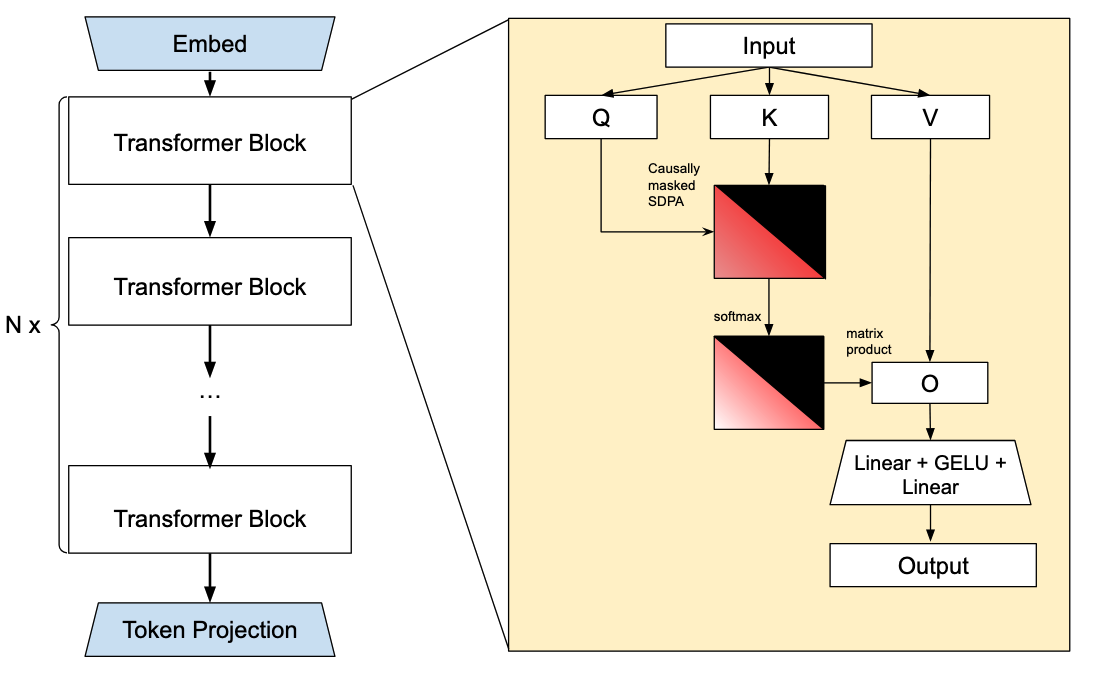
\includegraphics[width=0.45\textwidth, height=0.15\textheight]{images/gpt_arch.png}
    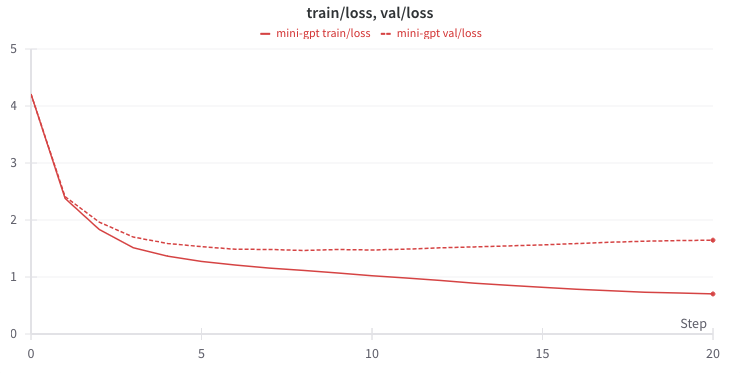
\includegraphics[width=0.45\textwidth, height=0.15\textheight]{images/loss_curves.png}
    \caption{(Left) The architecture of nanoGPT, illustrated. (Right) The training loss curves of the pre-trained nanoGPT model.}
    \label{fig:nanoGPT-sample}
\end{figure}
\begin{itemize}
    \item Despite being tokenized on a character level, the model could generate valid whole words
         with few to no errors.
    \item The model could generate text that (superficially) resembled the training corpus.
    \item The model often produced nonsensical text.
\end{itemize}


\section{Policy Gradient Algorithm}
\label{sec:alg-reinforce}

\begin{algorithm}[H] 
    \caption{Improved Policy Gradient Algorithm}
    \label{alg:reinforce}
    \begin{algorithmic}[1]
        \State Input: Policy $\pi_\theta$, learning rate $\alpha$, baseline of choice $b(s_t)$
        \State Output: Updated policy $\pi_\theta$
        \While{not converged}
            \State Sample a batch of trajectories $T$ from the policy $\pi_\theta$
            \For{each trajectory $T$ in the batch}
                \State Compute the rewards-to-go $R_t$ for each time step $t$ in the trajectory
                \State Compute the baseline $b(s_t)$ for each time step $t$ in the trajectory
                \State Estimate $\nabla_\theta J(\pi_\theta) \approx \frac{1}{m} \left(\sum_{t = 0}^{n} R_t - b(s_t)\right) \left( \sum_{t=0}^{n} \nabla_\theta \log(\pi_\theta(a_t | s_t)) \right)$
            \EndFor
            \State $\theta \leftarrow \theta + \alpha \nabla_\theta J(\pi_\theta)$
        \EndWhile
    \end{algorithmic}
\end{algorithm}

\end{document}